% ==============================================================================
% LAB 119
% UNDERSÖKNING AV RC-KRETS
% ------------------------
%
% Author:
% Jonas Sjöberg     <tel12jsg@student.hig.se>
% Oscar Wallberg    <tco13owg@student.hig.se>
%
% License:
% Creative Commons Attribution-NonCommercial-ShareAlike 4.0 International
% See LICENSE.md for full licensing information.
% ==============================================================================

\section{Uppmätning av Bode-diagram}\label{bode}

\subsection{Experimentuppställning}\label{}
% ------------------------------------------------------------------------------
En så kallad experimentplatta eller ``breadboard'' används för att konstruera
kretsen som illustreras i Figur~\ref{fig:rc-schema}.  \par För att generera en
sinusformad signal används signalgeneratorn \texttt{HP33120A}, vars utgång
kopplas genom en BNC-förgrening till oscilloskopet \texttt{Agilent 54621A} och
genom en BNC- banankontaktadapter, med ``banankablar'' till breadboardplattans
skruvterminaler.  \par Oscilloskopets första kanal visar signalen från kretsens
ingång, punkten \texttt{Vout} i Figur~\ref{fig:rc-schema}. Samma punkt utgör
signalgeneratorns utgång och vid några mätningar användes en T-koppling av
BNC-kablar för att mata signalgeneratorns utgång till både experimentkopplingen
och oscilloskopet.  En oscilloskopprob är ansluten till oscilloskopets andra
kanal. Proben kopplas till kretsens utgång, punkten \texttt{Vout} i
Figur~\ref{fig:rc-schema} med en oscilloskop-prob. Proben ställs till att dämpa
med en faktor av 10:1 och den vertikala skalan justeras en dekad nedåt, så att
båda kanalerna visas med samma skalfaktor.
\par Impedansskillnaden mellan signalgenerator kabel mot 


\begin{figure}\label{fig:rc-schema}
  \centering
  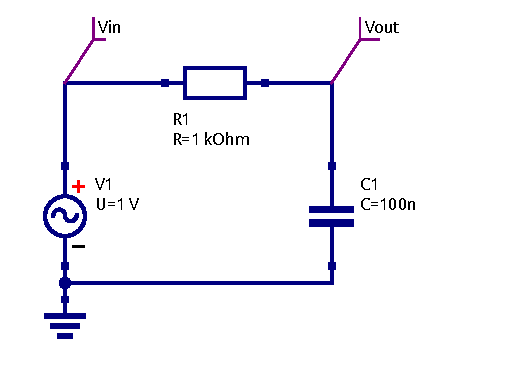
\includegraphics[width=0.8\linewidth]{sim/ee466_lab-4_prj/uppgift-0_schema}
  \caption[Schematisk ritning av labbkoppling, första ordningens RC-filter.]
  {Schematisk ritning av labbkoppling, första ordningens RC-filter.}
\end{figure}


\subsection{Beräkning}
% ------------------------------------------------------------------------------
Brytfrekvensen $f_1$ defineras som den frekvens då signalen har dämpats med
\SI{6}{\dB} och beräknas från ekv.~\eqref{eq:transfer2} enligt:

\begin{equation}\label{eq:cutoff}
  f_1 = \dfrac{1}{2 \pi R C} \si{\Hz}
\end{equation}

För kopplingen med komponentvärden enligt Figur~\ref{fig:rc-schema} beräknas
brytfrekvensen $f_1$ enligt ekv.~\eqref{eq:cutoff2}:

\begin{equation}\label{eq:cutoff2}
  \begin{split}
    f_1 &= \dfrac{1}{2    \pi \times \SI{1}{\kohm} \times \SI{100}{\nano\farad}} \si{\Hz} \\
        &= \dfrac{1}{2    \pi \times \num{1e3} \times \num{100e-6}}                       \\
        &= \dfrac{10^6}{2 \pi \times 10^3 \times \num{100}}                               \\
    f_1 &= \SI{1.591549431}{\Hz}
  \end{split}
\end{equation}

Vilket ger svaret i \eqref{eq:cutoff3}:

\begin{equation}\label{eq:cutoff3}
  \begin{split}
    f_1 &= \SI{1.591549431}{\Hz} \\
    f_1 &\approx \SI{1.592}{\Hz} \\
  \end{split}
\end{equation}


\subsection{Mätresultat}
% ------------------------------------------------------------------------------
% TODO: Lägg till faktiska mätresultat.

\begin{longtable}[c]{@{}ccccc@{}}
  \toprule\addlinespace
    \begin{tabular}{cc}$\text{Frekvens}        \\ (\si{\hertz})$   \end{tabular}
  & \begin{tabular}{cc}$U_{ut}                 \\ (\si{\volt})$    \end{tabular}
  & \begin{tabular}{cc}$U_{ut}/U_{in}          \\ (\si{\volt})$    \end{tabular}
  & \begin{tabular}{cc}$20 \log{U_{ut}/U_{in}} \\ (\si{\dB})$      \end{tabular}
  & \begin{tabular}{cc}$\phi                   \\ \text{(grader)}$ \end{tabular}
  \\\addlinespace
  \midrule\endhead
   100 & 2.11 & 1.01 & 5   \\\addlinespace
   300 & 2.06 & 0.99 & 10  \\\addlinespace
   500 & 2    & 0.96 & 17  \\\addlinespace
   700 & 1.94 & 0.93 & 24  \\\addlinespace
   900 & 1.84 & 0.88 & 29  \\\addlinespace
  1100 & 1.75 & 0.84 & 33  \\\addlinespace
  1300 & 1.66 & 0.79 & 37  \\\addlinespace
  1500 & 1.56 & 0.75 & 42  \\\addlinespace
  1700 & 1.49 & 0.71 & 45  \\\addlinespace
  1900 & 1.39 & 0.67 & 49  \\\addlinespace
  \bottomrule
  \addlinespace
  \caption[]{Mätresultat för kretsen i Figur~\ref{fig:rc-schema}.}
  \label{8a-table}
\end{longtable}

\subsection{Simulering}
% ------------------------------------------------------------------------------
För verifiering och visualisering av den teoretiska beräkningen körs en
\texttt{SPICE}-simulering av kretsen i det GPL-licensierade open source
programmet \texttt{Qucs}\footnote{\url{http://qucs.sourceforge.net/}}.
Simuleringsuppställningen och resultatet återfinns i
Figurer~\ref{fig:bode-sim-ac}, Figur~\ref{fig:bode-sim-tran} och
Figur~\ref{fig:bode-sim-param}.

\begin{figure}\label{fig:bode-sim-ac}
  \centering
  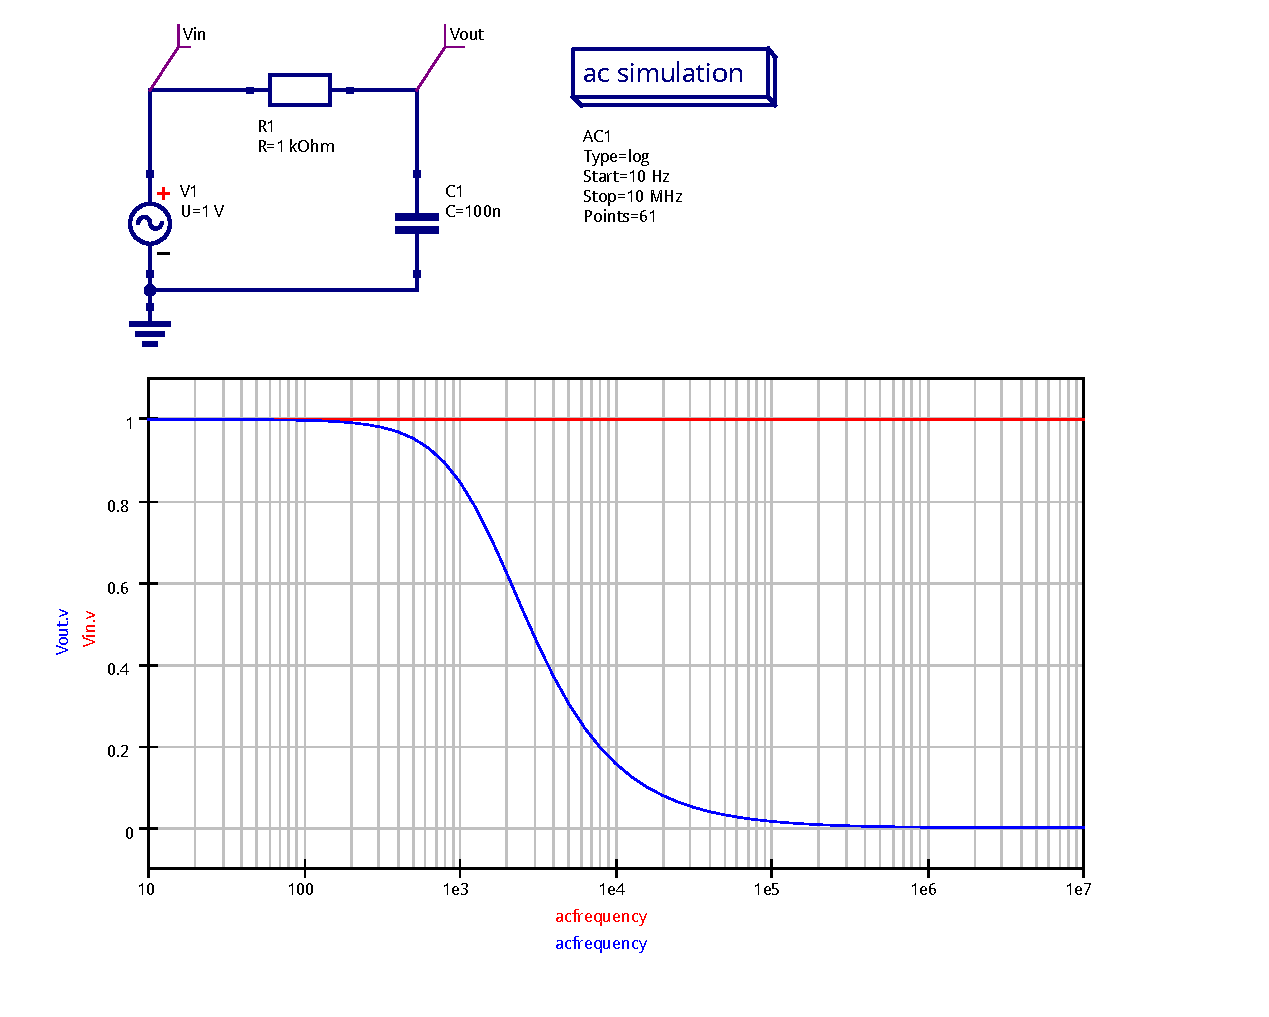
\includegraphics[width=\linewidth]{sim/ee466_lab-4_prj/uppgift-1_ac}
  \caption[] {Simulering av kretsens frekvensåtergivning.}
\end{figure}

\begin{figure}[ht]\label{fig:bode-sim-tran}
  \centering
  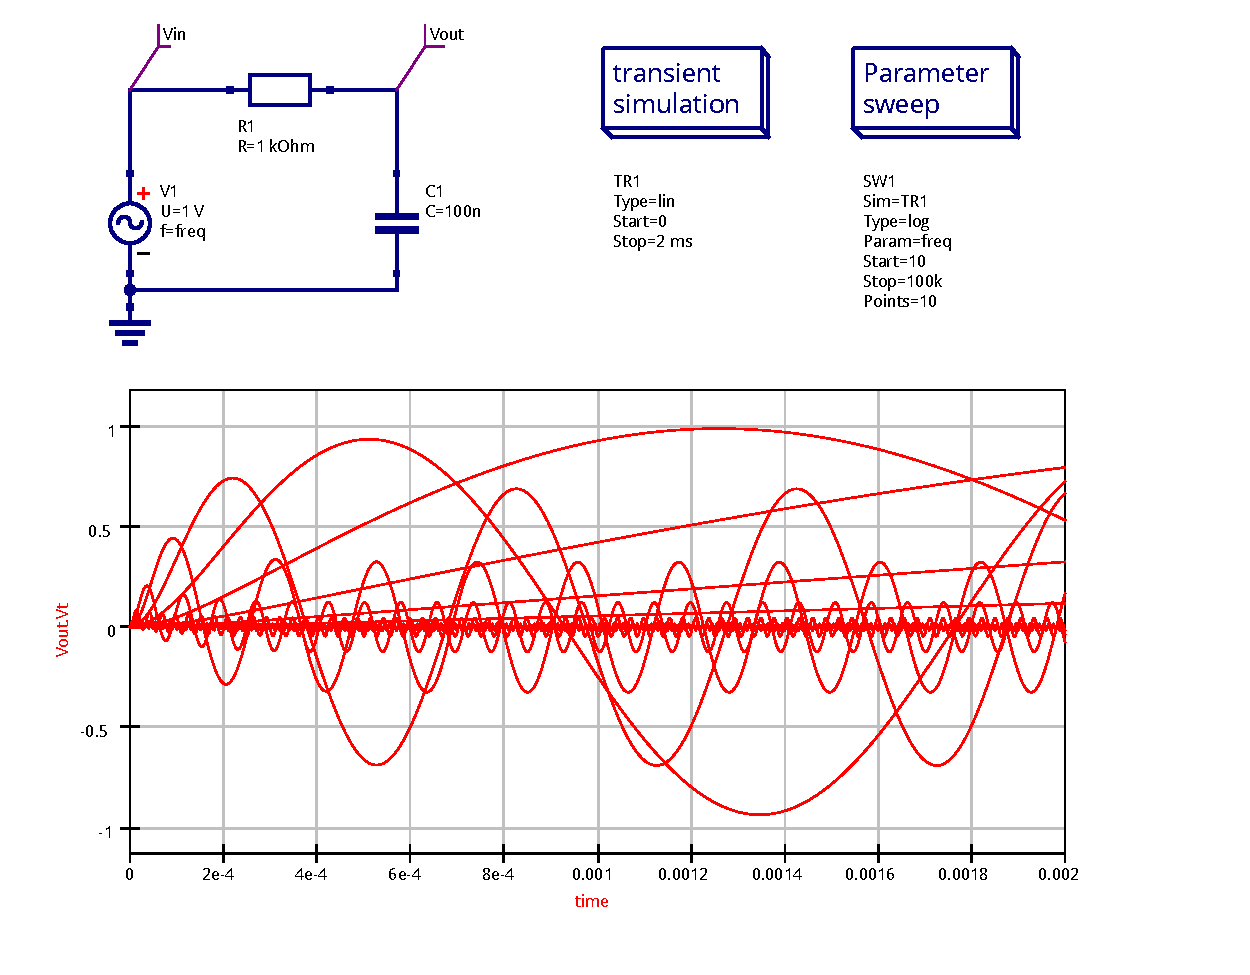
\includegraphics[width=\linewidth]{sim/ee466_lab-4_prj/uppgift-1_tran}
  \caption[] {Simulering av kretsen i tidsdomänen för olika frekvenser av $V_1$.}
\end{figure}

\begin{figure}[ht]\label{fig:bode-sim-param}
  \centering
  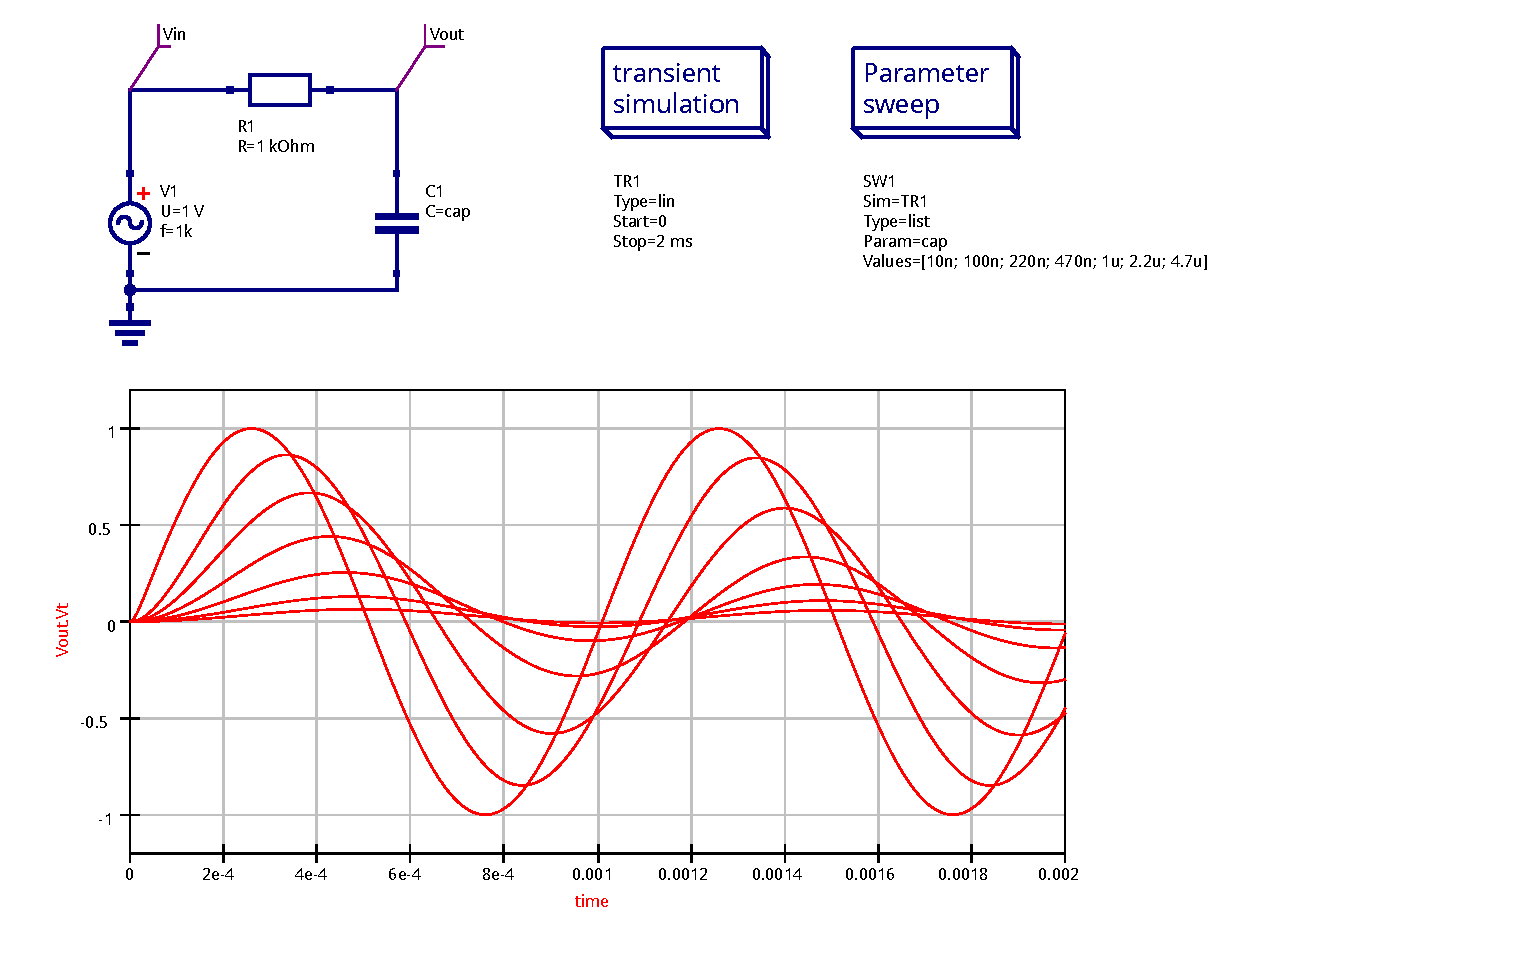
\includegraphics[width=\linewidth]{sim/ee466_lab-4_prj/uppgift-1_param}
  \caption[] {Simulering av kretsen i tidsdomänen för olika värden av $C_1$.}
\end{figure}


\subsection{Kommentar}\label{}
% ------------------------------------------------------------------------------
% TODO:


